\begin{frame}{Experimental Setup}
    Experiments presented in this paper were carried out using the Grid'5000 testbed, supported by a scientific interest group hosted by Inria and including CNRS, RENATER and several Universities as well as other organizations (see https://www.grid5000.fr).\\

    One evaluation on chuc cluster, using 4*A100 40G of VRAM GPU, is taking around 1 hour. Each algorithms have a budget of 50 evaluations, including the 10 sampling evaluation of BO. 

    \begin{block}{Hellaswag bounds}
        \begin{itemize}
            \item Upper bound : best accuracy on Hellaswag : 95.3\%. Done with GPT4 model, with 10-shot evaluation
            \item Lower bound : Sampling without exploitation : 55,7\%. Using one-shot LHS, with 10 picks to evaluate.
        \end{itemize}
        
        
    \end{block}
    
\end{frame}
%---------------------------------- Optimization -------------------------------
\begin{frame}[allowframebreaks]{BO}
    
    \begin{columns}
    
        \begin{column}{0.6\textwidth}
            \begin{block}{Score evolution}
                
                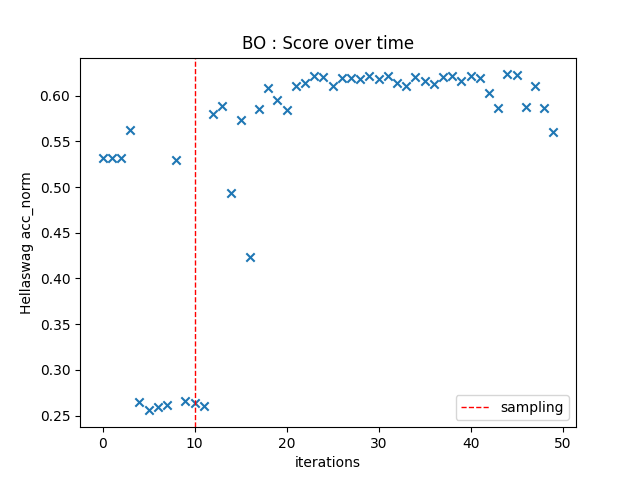
\includegraphics[width = 7.5cm]{imgs/plots/exp12_score_over_time.png}
            
            \end{block}   
        \end{column}

        \begin{column}{0.4\textwidth}
            \begin{block}{Results}
                Best score : 62.3\%               
            \end{block}
             
        \end{column}
    \end{columns}    


    \framebreak

    \begin{columns}
    
        \begin{column}{0.65\textwidth}
            \textbf{Score by variables and Varibles over iterations}
                \begin{figure}[h]
                    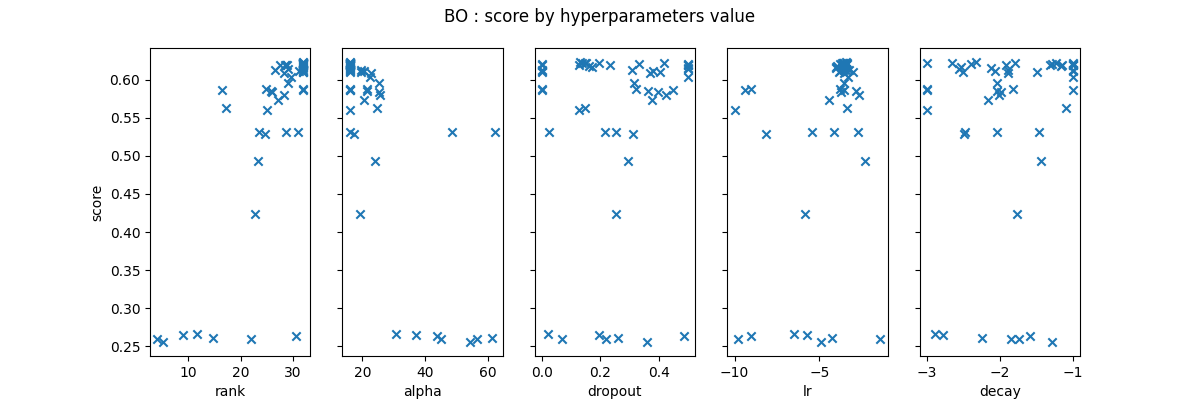
\includegraphics[width = \textwidth]{imgs/plots/exp12_score_by_hp.png}
                \end{figure}     
        \end{column}

        \begin{column}{0.4\textwidth}
            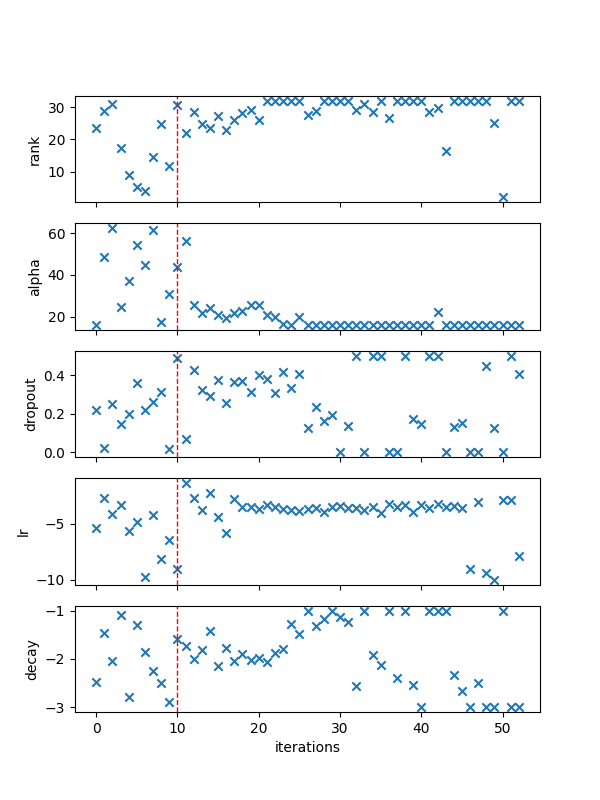
\includegraphics[height = 7cm]{imgs/plots/exp12_variables_over_time.png}
            
            
        \end{column}
    \end{columns}  
\end{frame}

%---------------------------------- Optimization -------------------------------
\begin{frame}[allowframebreaks]{SOO}
    
    \begin{columns}
    
        \begin{column}[t]{0.6\textwidth}
            \begin{block}{Score evolution}
                
                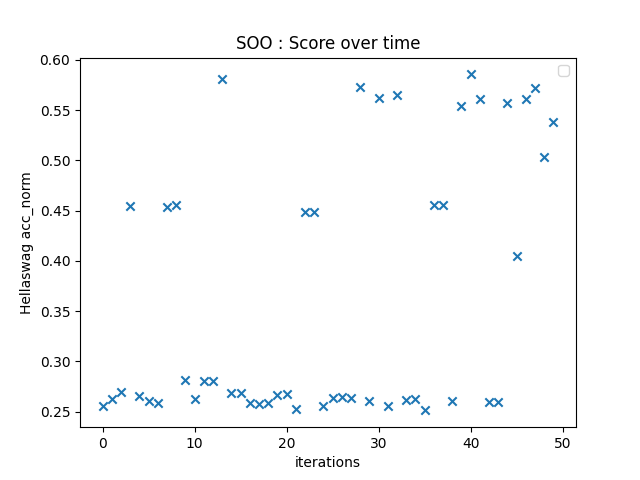
\includegraphics[width = 7.5cm]{imgs/plots/exp10_score_over_time.png}
            
            \end{block}   
        \end{column}

        \begin{column}[t]{0.4\textwidth}
            \begin{block}{Results}
                Best score : 58.4\%\\
                Slow convergence               
            \end{block}
            
            
        \end{column}
    \end{columns}   
    
    \framebreak

    \begin{columns}
    
        \begin{column}{0.65\textwidth}
            \textbf{Score by variables and Varibles over iterations}
                \begin{figure}[h]
                    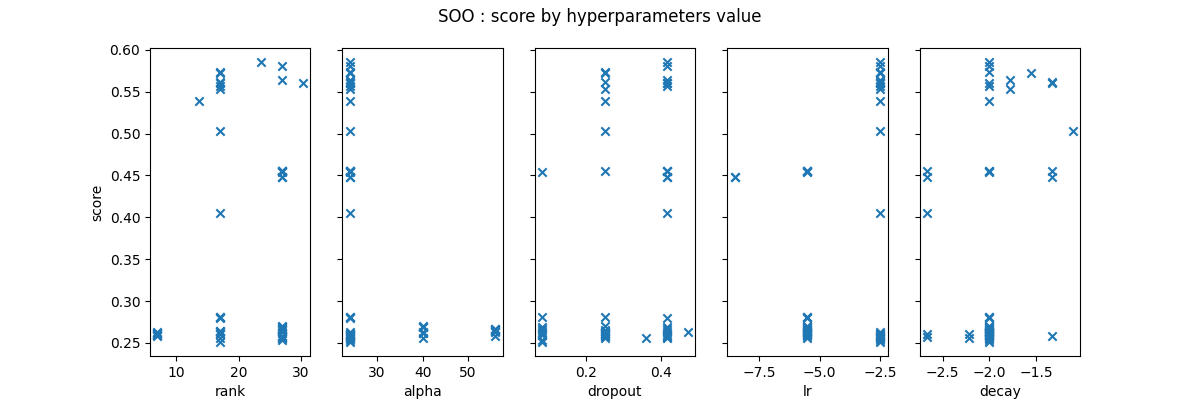
\includegraphics[width = \textwidth]{imgs/plots/exp10_score_by_hp.png}
                \end{figure}     
        \end{column}

        \begin{column}{0.4\textwidth}
            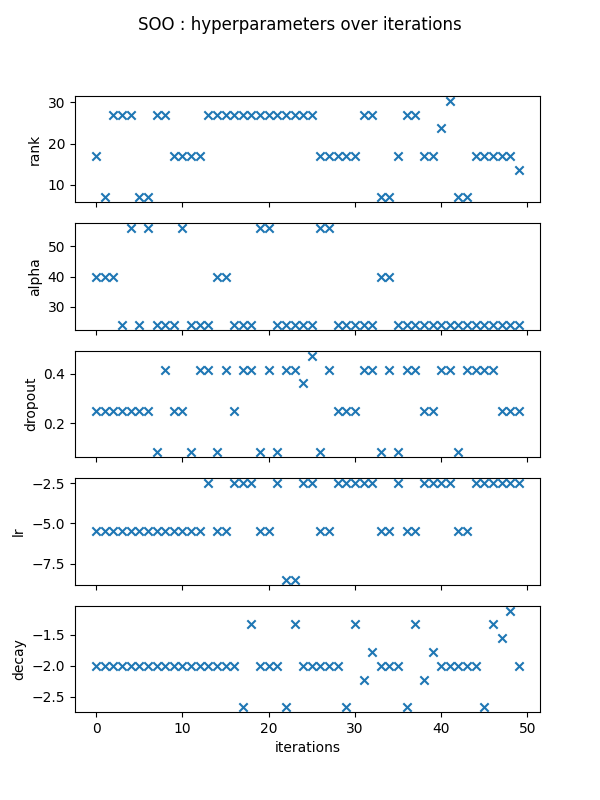
\includegraphics[height = 7cm]{imgs/plots/exp10_variables_over_time.png}
            
            
        \end{column}
    \end{columns}  
\end{frame}

%---------------------------------- Optimization -------------------------------
\begin{frame}[allowframebreaks]{BaMSOO}
    
    \begin{columns}
    
        \begin{column}[t]{0.6\textwidth}
            \begin{block}{Score evolution}
                
                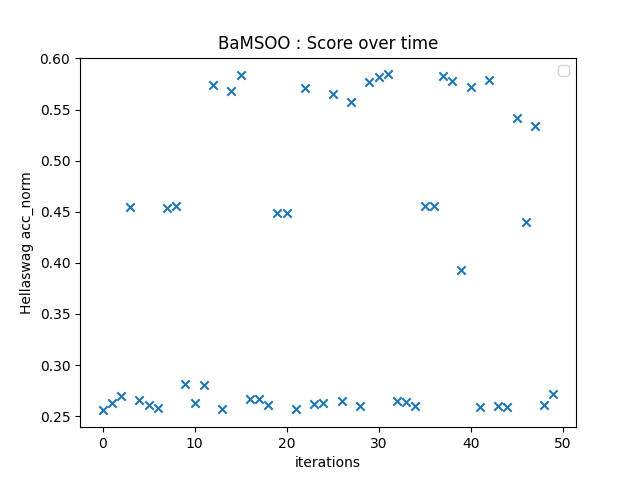
\includegraphics[width = 7.5cm]{imgs/plots/exp11_score_over_time.png}
            
            \end{block}   
        \end{column}

        \begin{column}[t]{0.4\textwidth}
            \begin{block}{Results}
                Best score : 58.5\%\\
                Not so much approximations, need to increase $\eta $ in equation \ref{eq:ucb} to speed the convergence              
            \end{block}
            
            
        \end{column}
    \end{columns}    

    \framebreak

    \begin{columns}
    
        \begin{column}{0.65\textwidth}
            \textbf{Score by variables and Varibles over iterations}
                \begin{figure}[h]
                    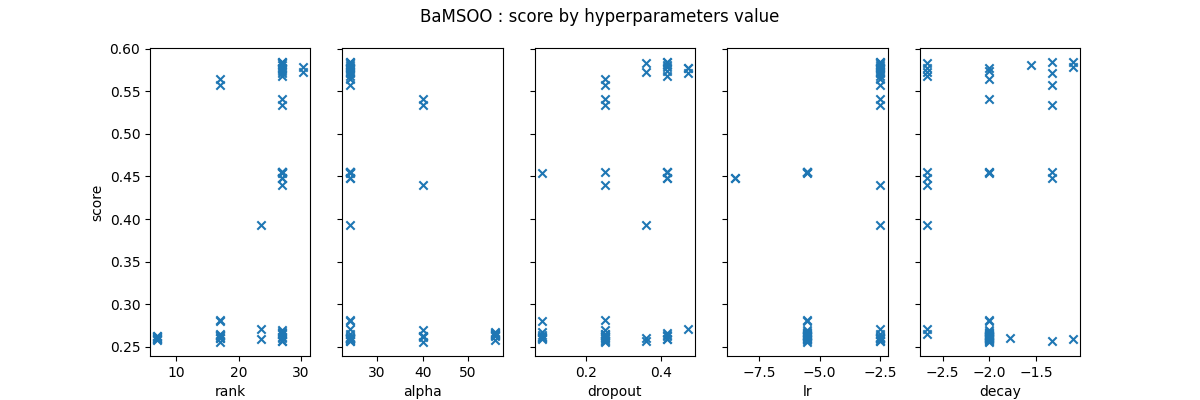
\includegraphics[width = \textwidth]{imgs/plots/exp11_score_by_hp.png}
                \end{figure}     
        \end{column}

        \begin{column}{0.4\textwidth}
            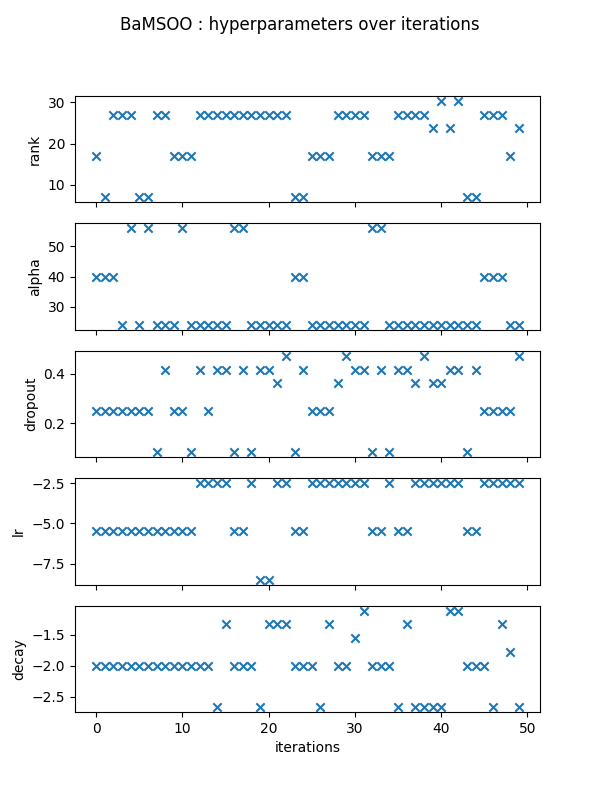
\includegraphics[height = 7cm]{imgs/plots/exp11_variables_over_time.png}
            
            
        \end{column}
    \end{columns}  
\end{frame}
